\documentclass[10pt]{beamer}

%%%
% PREAMBLE FOR THIS DOC 
%%%
%https://tex.stackexchange.com/questions/68821/is-it-possible-to-create-a-latex-preamble-header
\usepackage{/Users/miw267/Repos/latex_preamble/beamer_preamble}


%%%
% PREAMBLE SPECIAL FOR THIS DECK
%%%
\definecolor{condred}{RGB}{200,30,30}
\definecolor{accessgreen}{RGB}{30,160,60}
\usetikzlibrary{calc}


%%%
% AGENDA TOPICS
%%%
\agendatopic[motivation]{Motivation}
\agendatopic[logic]{Logic}
\agendatopic[if-then]{If-then statements}
\agendatopic[if-and-only-if]{If-and-only-if statements}
%\agendatopic[quiz-solution]{Solution to practice quiz}
\agendatopic[big-picture]{The big picture: propositional logic}
%\agendatopic[group-exercises]{Group exercises}


\lstset{
  language=Python,
  backgroundcolor=\color{black!5},
  keywordstyle=\color{blue}\bfseries,
  stringstyle=\color{orange},
  commentstyle=\color{green!60!black},
  basicstyle=\ttfamily\small,
  numbers=left,
  numberstyle=\tiny\color{gray},
  frame=single,
  showstringspaces=false
}

%%%
% DOCUMENT
%%%

\begin{document}






\title{Monday 08/31/2026: Theorems}
\author{CSCI 246: Discrete Structures}
\date{Textbook reference: Sec. 4, Scheinerman}


\begin{frame}
    \titlepage 
\end{frame}


\begin{frame}

\begin{mygreenbox}[title=Logistical Matters]
\begin{itemize}
\item \textbf{Reminder:} Your two jobs before each class are to (a) make sure you can do all the group exercises and (b) read the next section (see syllabus).  
\item \textbf{Office Hours:} My and Madhav's office hours have been posted to the syllabus.
\item \textbf{Weekly Quiz:} This Friday's weekly quiz will have three questions, and will cover definitions and theorems.
	\begin{center}
	
\includegraphics[width=.8\textwidth]{images/weekly_quizzes}	
	\end{center}
\end{itemize}
\end{mygreenbox}

\vfill 


\begin{myyellowbox}[title=Today's Agenda]
\begin{itemize}
	\item Mini lecture ($\approx$ 35 mins)
	\item Group exercises ($\approx$ 15 mins)
\end{itemize}


\end{myyellowbox}
\vfill 

\end{frame}

\agendaframe{motivation}


\begin{frame}[standout]
Why care about theorems?	
\end{frame}

\begin{frame}{Shrinking data without losing distances}

%\begin{evidence}[blue]
%\textbf{Applied Problem.}  Every Netflix user is a vector of \textbf{50,000} movie ratings.  To find similar users, \textit{each} distance you compute costs 50,000 operations. \blue{\textbf{Can you shrink the vectors and still find similar users?}}
%\end{evidence}

\begin{evidence}[blue]
\begin{minipage}[c]{0.84\linewidth}
\textbf{Applied Problem.}  Every Netflix user is a vector of \textbf{50,000} movie ratings.  To find similar users, \textit{each} distance you compute costs 50,000 operations. \blue{\textbf{Can you shrink the vectors and still find similar users?}}
\end{minipage}\hfill
\begin{minipage}[c]{0.13\linewidth}

\includegraphics[width=\linewidth]{images/netflix}
\end{minipage}
\end{evidence}

\pause
\vspace{-.2cm}

\begin{evidence}[red]
\textbf{Possible Solutions.}	
\vspace{-.2cm}
\begin{itemize}
\item \textit{Drop coordinates?}  \pause  Two users differing \textbf{\red{only}} in the
      dropped ones now look identical.
\item \textit{Keep the most informative ones?} \pause   To decide which, you must
      examine \textbf{\red{all}} the data, the thing you were avoiding.
\end{itemize}
\end{evidence}

\pause
\vspace{-.2cm}

\begin{evidence}[green]
\textbf{{Johnson--Lindenstrauss Theorem (informally)}} Take \textit{any} $n$ points in $\R^d$.   \pause 
	Multiply them all by a \textbf{\forestgreen{random}} matrix that squashes them down to $k \approx (\log n)/\varepsilon^2$ dimensions. \pause 
	With high probability, \textbf{\forestgreen{every}} pairwise distance is preserved to within a
factor of $1 \pm \varepsilon$.
\end{evidence}

\pause
\vspace{-.2cm} 

\begin{evidence}[orange]
\textbf{Remark.}	 This solution doesn't require looking at the data \textbf{at all!}
\end{evidence}

%$k$ depends on the \textbf{number of points} and the \textbf{accuracy} --- \textbf{not} on $d$.}

\end{frame}


\begin{frame}{Why care about theorems?}


{\large\textbf{Pipeline for building a malware detector}}
\begin{center}
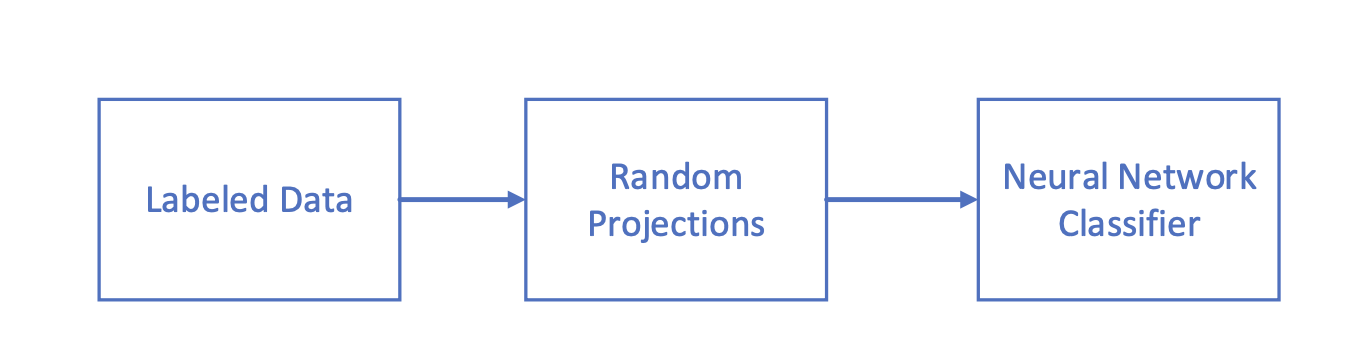
\includegraphics[width=0.68\textwidth]{images/malware_detection_via_RPs}
\end{center}
\evsrc{\hfill Dahl, Stokes, Deng \& Yu, ``Large-scale malware classification using
random projections and neural networks,'' \textit{IEEE ICASSP}, 2013.}

\vfill
{\color{black!25}\rule{\linewidth}{0.6pt}}
\vspace{0.3em}
\pause 
%
%\pause
%{\large\textbf{Why care about theorems?}}
%\pause 
\vspace{0.2em}
\begin{center}
\begin{tikzpicture}
  % the executive
  \node[anchor=west, inner sep=0pt, draw=black!25, line width=0.4pt]
       (mike) at (-0.5,0) {
\includegraphics[height=3cm]{images/mike_scott}};
  % the speech bubble (drawn first, so the tail fill can cover its left border)
  \node[draw=black!45, fill=blue!6, rounded corners=4pt, anchor=west,
        text width=6.1cm, align=left, inner sep=8pt] (bub) at (2.75,0.42)
       {Make the dimensionality reduction better! It's \textbf{random}!};
  % the tail
  \fill[blue!6]   (2.75,0.62) -- (2.35,0.42) -- (2.75,0.23) -- cycle;
  \draw[black!45] (2.75,0.62) -- (2.35,0.42) -- (2.75,0.23);


  % freeze the extent of everything above, then strike it out
  \coordinate (xSW) at (current bounding box.south west);
  \coordinate (xNE) at (current bounding box.north east);
  \coordinate (xNW) at (current bounding box.north west);
  \coordinate (xSE) at (current bounding box.south east);
  \only<3->{\draw[red, line width=4pt, opacity=0.8, line cap=round]
              (xSW) -- (xNE)  (xNW) -- (xSE);}
              
\end{tikzpicture}
\end{center}

\end{frame}



\agendaframe{logic}

\begin{frame}{Logic}

\begin{columns}[T,onlytextwidth]

\begin{column}{0.61\textwidth}
The statements in a theorem are written in a \textbf{formal language}.
Its vocabulary is tiny: a handful of \alert{logical connectives}:

\vspace{0.7em}
{\centering
\begin{tabular}{@{}l@{\hspace{1.4em}}c@{}}
\textbf{and}             & $\land$    \\[4pt]
\textbf{or}              & $\lor$     \\[4pt]
\textbf{not}             & $\lnot$    \\[4pt]
\textbf{if--then}        & $\implies$ \\[4pt]
\textbf{if and only if}  & $\iff$     \\
\end{tabular}\par}

\vspace{0.9em}
{\small Also called \textbf{logical operators},  the same things your programming language spells \texttt{\&\&}, \texttt{||}, \texttt{!}.}
\end{column}

\begin{column}{0.35\textwidth}
\centering
\fcolorbox{black!25}{white}{
\includegraphics[width=0.88\linewidth]{images/logic}}

\vspace{0.4em}
\textit{Logic (the rapper)}
\end{column}

\end{columns}
\end{frame}

\begin{frame}{Practice Quiz on Reading}

Replace each $\red{?}$ with a checkmark \greencheck if the combination of truth values for propositions A and B is \textit{possible} under the given logical connective.  Replace it with a \redx if the combination is \textit{impossible}.
% IE we want to know if it violates the logical rule.

\begin{table}
\centering
\begin{tabular}{cc|ccc}
\multicolumn{2}{c}{\textbf{Propositions}} & \multicolumn{3}{c}{\textbf{Logical connective}} \\
A  & B & if A then B & if B then A & A if and only if B \\
\hline 
T & T & \red{?} & \red{?} & \red{?}\\
T & F &\red{?}  & \red{?} & \red{?} \\
F & T & \red{?} & \red{?} & \red{?} \\
F & F & \red{?} &\red{?}  & \red{?}
\end{tabular}
\end{table}

\pause 
\begin{center}
\bluetextbox{The goal of today's slides is to clarify the solution.}	
\end{center}

\end{frame}

%%%%%%%%%%%%%%%%%%%%%%
\agendaframe{if-then} 


\begin{frame}{If-then: Truth Table}
\label{slide:truth_table_for_if_A_then_B}
Given two propositions $A$ and $B$, the new proposition \qq{If A, then B} ($A  \implies B$) can be written in terms of this  \textit{truth table}:

\begin{center}
\begin{tabular}{cc|c}
A & B & $\overbrace{A \implies B}^{\text{If A, then B}}$ \\
\hline 
T & T & \green{T} \\
T & F & \red{F} \\
F & T & \green{T}  \\
F & F & \green{T}  \\
\end{tabular}
\end{center}
\vfill
The green rows are \forestgreen{consistent} with the statement, and the red rows \red{violate} it.
\pause  
\vfill 
\colorbox{blue!30}{\textbf{Summary.}} If A is True, B \alert{must} be True. 
\pause  
\vfill  
\colorbox{yellow!30}{\textbf{Remark.}}  If A is False, then no restrictions are placed on B.
\pause  
\vfill
%\colorbox{green!30}{\textbf{Example.}} Let $A$ = \texttt{A person lives in Bozeman}, $B$ = \texttt{The person lives in Montana}.  Here, $A \implies B$.  (Check this against the truth table; give an example for each row.)
\colorbox{green!30}{\textbf{Example.}} Let $A$ = \texttt{A person lives in Bozeman}, $B$ = \texttt{The person lives in Montana}.  Let's check this against the truth table, row by row.
\end{frame}


\begin{frame}{If-then: Example}

Let $A$ = \texttt{A person lives in Bozeman} and $B$ = \texttt{The person lives in Montana}.

\vfill
\begin{center}
\begin{tabular}{cc|c|l}
A & B & $\overbrace{A \implies B}^{\text{If A, then B}}$ & Example \\
\hline
T & T & \forestgreen{T} & \makebox[4.4cm][l]{\only<2->{\forestgreen{Me}}} \\[2pt]
T & F & \red{F}   & \makebox[4.4cm][l]{\only<3->{\red{\textbf{Not possible!}}}} \\[2pt]
F & T & \forestgreen{T} & \makebox[4.4cm][l]{\only<4->{\forestgreen{Justin Timberlake}}} \\[2pt]
F & F & \forestgreen{T} & \makebox[4.4cm][l]{\only<5->{\forestgreen{Taylor Swift}}} \\
\end{tabular}
\end{center}

\vfill
\only<6->{\colorbox{blue!30}{\textbf{Conclusion.}} The only row that would
\red{violate} the rule (Bozeman but not Montana) \textbf{cannot happen}.
Therefore $A \implies B$.}

\end{frame}


\begin{frame}{If-then: Set Theoretic Perspective}
Let \gold{$A$} = \texttt{A person lives in Bozeman} and \blue{$B$} = \texttt{The person lives in Montana}.   Then $A \implies B$!

\begin{columns}[T] % align columns at the top

% Left column: TikZ diagram
\begin{column}{0.6\textwidth}
\begin{center}
\begin{tikzpicture}[scale=0.625]
% Draw outer shape B
\draw[thick, blue] (0,0) ellipse (4.5cm and 3cm) node[above=2cm] {Live in Montana};

% Draw inner shape A
\draw[thick, gold] (0,0) ellipse (2cm and 1.2cm) node[above=1cm] {Live in Bozeman};

% Points inside A
\fill (0.5,-0.4) circle (2pt);
\fill (-0.1,0.0) circle (2pt);
\fill (1,-0.8) circle (2pt);
\node[above] at (-0.1,0.0) {Brock Tessman}; % labeled point inside A

% Points inside B but not A
\fill (2.5,0.5) circle (2pt);
\fill (-2.8,-0.5) circle (2pt);
\fill (1.8,-1.8) circle (2pt);
\node[above] at (1.8,-1.8) {Justin Timberlake}; % labeled point in B but not A

% Points outside B
\fill (-5,-1.5) circle (2pt);
\fill (0,-3.5) circle (2pt);
\node[below] at  (-5,-1.5) {Taylor Swift}; % labeled point outside B

\end{tikzpicture}
\end{center}
\end{column}

% Right column: Justin Timberlake picture
\begin{column}{0.4\textwidth}
\begin{center}

\includegraphics[width=\textwidth]{images/jt}	
\end{center}
\end{column}
\end{columns}


\vfill 
\pause 


\vfill  
\colorbox{yellow!30}{\textbf{Set theoretic perspective.}}  You can think about $A \implies B$ as \qq{the set of things satisfying property $A$ is contained within the set of things satisfying property $B$.}

\end{frame}


% Now we install the new template for the following frames:
{\usebackgroundtemplate{%
  
\includegraphics[width=\paperwidth,height=\paperheight]{images/flying_elephant}} 
\begin{frame}
\centering 
\Large \color{black} \textbf{Poll: True or False?} Every elephant flying with polka-dotted balloons above Bozeman is smoking a cigar. \color{black}
\vfill \vfill \vfill \vfill 
\end{frame}
}


\begin{frame}{Vacuous Truths}

\small 
\begin{mygreenbox}[title=Solution to poll]
Let $A$ = \texttt{this is an elephant flying with polka-dotted balloons above Bozeman} and $B$ = \texttt{this is smoking a cigar}.  Then $A$ is always False. So $A \implies B$ is \alert{TRUE!!!} This is called a \textbf{vacuous truth.}  Per Scheinerman, these statements are true \qq{because they have no exceptions.}
\end{mygreenbox}

\pause  
\vfill 

\begin{myyellowbox}[title=Reference material]
Given two propositions $A$ and $B$, the statement \qq{If A, then B} ($A  \implies B$) holds whenever following \qq{truth table} applies:

\begin{center}
\begin{tabular}{cc|c}
A & B & $\overbrace{A \implies B}^{\text{If A, then B}}$ \\
\hline 
T & T & \green{T} \\
T & F & \red{F} \\
F & T & \green{T}  \\
F & F & \green{T}  \\
\end{tabular}
\end{center}
\end{myyellowbox}

\end{frame}



\begin{frame}{If-then: Valid argument and logical fallacy}

% First green box
\begin{mygreenbox}[title=\textit{Modus Ponens} (A valid argument) \greencheck]
    \begin{minipage}[t]{0.35\linewidth}
    \textbf{Structure} \\
       If A, then B. \\
       A. \\
       Therefore B.
    \end{minipage}\hfill
    \begin{minipage}[t]{0.60\linewidth}
    \textbf{Example} \\
       If it is raining, the ground is wet. \\
       It is raining. \\
       Therefore, the ground is wet.
    \end{minipage}
\end{mygreenbox}

\vspace{0.5cm}
\pause 

\begin{myredbox}[title=\textit{Affirming the Consequent} (A logical fallacy) \redx]
    \begin{minipage}[t]{0.35\linewidth}
    \textbf{Structure} \\
       If A, then B. \\
       B. \\
       Therefore A.
    \end{minipage}\hfill
     \begin{minipage}[t]{0.60\linewidth}
    \textbf{Example} \\
       If it is raining, the ground is wet. \\
       The ground is wet. \\
       Therefore, it is raining.
    \end{minipage}
\end{myredbox}

\end{frame}



\begin{frame}{If-then: Other jargon}

Some other terminology which means the same thing:
\begin{itemize}
\item A implies B
\item A is sufficient for B
\item B is necessary for A (A "only if" B)
\end{itemize}
 
	
\end{frame}


%%%%%%%%%%%%%%%%%%%%%%
\agendaframe{if-and-only-if}

\begin{frame}{If and only if: Definition and shorthand}

\only<1>{
\begin{mygreenbox}[title=\textit{If and only if} statements: Definition]

\[ \explaintermbrace{A if and only if B}{A \iff B} \quad \text{means} \quad \explaintermbrace{if A then B}{(A \implies B)} \; \texttt{and} \; \explaintermbrace{if B then A}{(A  \impliedby B)} \] 
\end{mygreenbox}
}

\only<2->{
\begin{mygreenbox}[title=\textit{If and only if} statements: Definition]

\[ \explaintermbrace{A if and only if B}{A \iff B} \quad \text{means} \quad \explaintermbrace{A only if B}{(A \implies B)} \; \texttt{and} \; \explaintermbrace{A if B}{(A  \impliedby B)} \] 
\end{mygreenbox}
}



\only<3->{
\colorbox{red!30}{\textbf{Shorthand.}}  For convenience, we can abbreviate \texttt{A if and only if B} as \texttt{A iff B}.
}
\end{frame}


\begin{frame}{If and only if: Truth Table}
\footnotesize
 The truth table for the ``\texttt{and}" operator (also written $\land$) is given by  
\begin{center}
\begin{tabular}{cc|c}
\multicolumn{2}{c}{\textbf{Original propositions}} & \multicolumn{1}{c}{\textbf{New proposition}} \\
X & Y & $X \land Y$ \\
\hline 
T & T & T \\
T & F & F \\
F & T & F  \\
F & F & F  \\
\end{tabular}
\end{center}
\pause 
Now we apply the $\land$ operator to the results of the $\implies$ and $\impliedby$ operators.
 
\begin{table}
\centering
\begin{tabular}{cc|ccc}
\multicolumn{2}{c}{\textbf{Orig. props.}} & \multicolumn{3}{c}{\textbf{New props.}} \\
A & B & $\overbrace{A \implies B}^{X}$  & $\overbrace{B \implies A}^{Y}$& $\overbrace{(A \implies B) \land  (B \implies A)}^{X \land Y}$ \\
\hline 
T & T & \green{T}  & \green{T} & \green{T}\\
T & F & \red{F} & \green{T} &  \red{F}  \\
F & T & \green{T}  &  \red{F}  &  \red{F}  \\
F & F & \green{T} & \green{T} & \green{T}
\end{tabular}
\end{table}

\end{frame}

\begin{frame}{If and only if: Truth Table}

Given two propositions $A$ and $B$, the statement \qq{A if and only if B} (that is, the property $A  \iff B$) holds whenever following \qq{truth table} applies:

\begin{center}
\begin{tabular}{cc|c}
A & B & $\overbrace{A \iff B}^{\text{A if and only if B}}$ \\
\hline 
T & T & \green{T} \\
T & F & \red{F} \\
F & T & \red{F}  \\
F & F & \green{T}  \\
\end{tabular}
\end{center}
\pause  
\vfill 
\colorbox{blue!30}{\textbf{Summary.}} A and B are \underline{both} True or \underline{both} False.
\pause  
\vfill  
\colorbox{green!30}{\textbf{Example.}} Let $A$ = \texttt{This month contains Labor Day}, $B$ = \texttt{This month is September}.  Let's check this against the truth table, row by row.
\end{frame}




\begin{frame}{If-then: Example}

Let $A$ = \texttt{This month contains Labor Day} and $B$ = \texttt{This month is September}.

\vfill
\begin{center}
\begin{tabular}{cc|c|l}
A & B & $\overbrace{A \iff B}^{\text{A if and only if B}}$ & Example \\
\hline
T & T & \forestgreen{T} & \makebox[4.4cm][l]{\only<2->{\forestgreen{September 2021}}} \\[2pt]
T & F & \red{F}   & \makebox[4.4cm][l]{\only<3->{\red{\textbf{Not possible!}}}} \\[2pt]
F & T & \red{F} & \makebox[4.4cm][l]{\only<4->{\red{\textbf{Not possible!}}}} \\[2pt]
F & F & \forestgreen{T} & \makebox[4.4cm][l]{\only<5->{\forestgreen{April 2026}}} \\
\end{tabular}
\end{center}

\vfill
\only<6->{\colorbox{blue!30}{\textbf{Conclusion.}} The only rows that would
\red{violate} the rule  \textbf{cannot happen}.
Therefore $A \iff B$.}

\end{frame}

\begin{frame}{If and only if: Set theoretic perspective}
Let \red{$A$} = \texttt{This month contains Labor Day} and \blue{$B$} = \texttt{This month is September}.   Then $A \iff B$!

\begin{center}
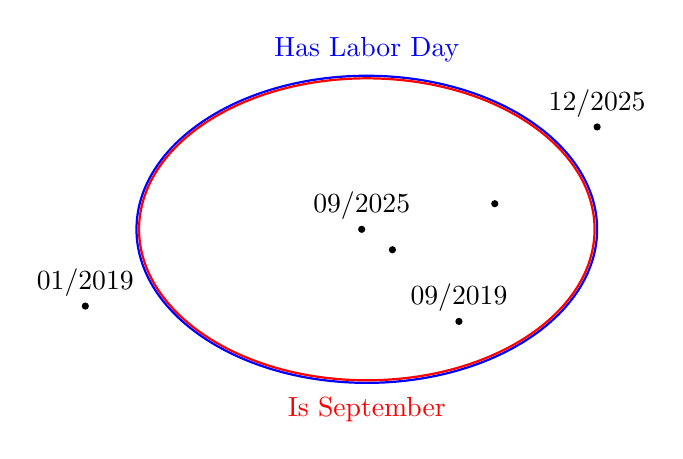
\begin{tikzpicture}[scale=0.65]
% Draw outer shape B
\draw[thick, blue] (0,0) ellipse (4.5cm and 3cm) node[above=2cm] {Has Labor Day};

% Draw inner shape A
\draw[thick, red] (0,0) ellipse (4.45cm and 2.95cm) node[below=2cm] {Is September};

% Points inside A and B
\fill (0.5,-0.4) circle (2pt);
\fill (2.5,0.5) circle (2pt);
\fill (-0.1,0.0) circle (2pt);
\fill (1.8,-1.8) circle (2pt);
\node[above] at (-0.1,0.0) {09/2025}; % labeled point inside A
\node[above] at (1.8,-1.8) {09/2019}; % labeled point in B but not A

% Points outside B
\fill (4.5,2) circle (2pt);
\fill (-5.5,-1.5) circle (2pt);
\node[above] at (4.5,2) {12/2025}; % labeled point outside B
\node[above] at (-5.5,-1.5) {01/2019}; % labeled point outside B

\end{tikzpicture}
\end{center}
\vfill 
\pause 

 \vfill  
\colorbox{yellow!30}{\textbf{Set theoretic perspective.}}  You can think about $A \iff B$ as \qq{the set of things satisfying property $A$ is identical to the set of things satisfying property $B$.}

\end{frame}
%
%\begin{frame}{If and only if: Big picture}
%
% $A \iff B$  means that $A$ and $B$ are just two different descriptions of the same thing!
% 	
%\end{frame}


\begin{frame}{If and only if: Big picture}
\centering
\vfill
{\color{gold}\faStar\;\faStar\;\faStar}

\vspace{0.7em}
{\LARGE $A \iff B$}

\vspace{1.2em}
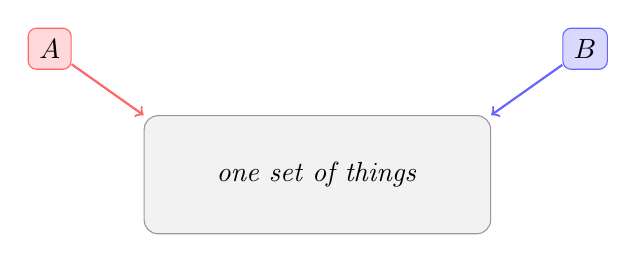
\begin{tikzpicture}
  \node[draw=black!40, fill=black!5, rounded corners=5pt, minimum width=4.4cm,
        minimum height=1.5cm, align=center] (thing) at (0,0)
        {\textit{one set of things}};
  \node[fill=red!15, draw=red!60, rounded corners=3pt, inner sep=4pt] (a) at (-3.4,1.6) {\red{$A$}};
  \node[fill=blue!15, draw=blue!60, rounded corners=3pt, inner sep=4pt] (b) at (3.4,1.6) {\blue{$B$}};
  \draw[->, thick, red!60]  (a) -- (thing.north west);
  \draw[->, thick, blue!60] (b) -- (thing.north east);
\end{tikzpicture}

\vspace{1.0em}
{\large $A$ and $B$ are two different \textbf{descriptions} of the \gold{\textbf{same thing}}.}
\vfill
\end{frame}

\begin{frame}[fragile]{If and only if: Why should computer scientists care?}

Consider the following theorem.
\vfill 
\begin{mygreenbox}[title=\textbf{Theorem (Graph Theory)}]
A connected undirected graph with $n$ vertices has a cycle if and only if it has at least $n$ edges.	
\end{mygreenbox}
\vfill 

Thanks to the \qq{iff}, you know that edge count alone is enough to decide whether a cycle exists.  Instead of running a full DFS or Union-Find cycle detection algorithm, you can just check counts:

\vfill 

\begin{lstlisting}
def has_cycle(num_vertices, edges):
    return len(edges) >= num_vertices
\end{lstlisting}

\vfill \pause 

\colorbox{red!30}{\textbf{Take home.}}  Why would computer scientists care about theorems of the  form \qq{A iff B}?  It can sometimes happen that what we really want is A, but that’s very hard to code up.  Thanks to the theorem, we can just code up B instead, because it turns out (perhaps surprisingly!) that it's the exact same thing.
\end{frame}




%\agendaframe{quiz-solution}







%%%%%%%%%%%%%%%%%%%%%%
\agendaframe{big-picture}



\begin{frame}{Solution to practice quiz}
\small 
\begin{table}
\centering
\begin{tabular}{cc|ccc}
\multicolumn{2}{c}{} & \multicolumn{3}{c}{} \\
A  & B & if A then B & if B then A & A if and only if B \\
\hline 
T & T & \green{T}  & \green{T} & \green{T}\\
T & F & \red{F} & \green{T} &  \red{F}  \\
F & T & \green{T}  &  \red{F}  &  \red{F}  \\
F & F & \green{T} & \green{T} & \green{T}
\end{tabular}
\end{table}
\end{frame}

\begin{frame}{Propositional logic}
\label{slide:prop_logic}
\small 
\begin{table}
\centering
\begin{tabular}{cc|ccc}
\multicolumn{2}{c}{\textbf{Original propositions}} & \multicolumn{3}{c}{\textbf{New propositions}} \\
A  & B & if A then B & if B then A & A if and only if B \\
\hline 
T & T & \green{T}  & \green{T} & \green{T}\\
T & F & \red{F} & \green{T} &  \red{F}  \\
F & T & \green{T}  &  \red{F}  &  \red{F}  \\
F & F & \green{T} & \green{T} & \green{T}
\end{tabular}
\end{table}
\pause 
\vfill 
\begin{itemize}
\item The column headings show 3 new propositions, formed from the original propositions by \textbf{logical operators}. \pause 
\item Each logical operator can be thought of as a \textbf{function} or mapping $\set{T,F} \times \set{T,F} \to \set{T,F}$.  \pause 
\item Besides \texttt{if-then} and \texttt{if-and-only-if}, there are other logical operators (\texttt{and, or, xor}, etc.), some of which were discussed in the text. \pause 
\item The study of how to combine and change propositions under logical operators to form more complex propositions is called \textbf{propositional logic}. 
\end{itemize}

\vfill \pause 
\colorbox{yellow!30}{\textbf{Terminology.}} The first two columns combined with one remaining column gives the \alert{\textbf{truth table}} for that logical operator. 
\end{frame}


\begin{frame}{Why are we doing all of this?}


\colorbox{red!30}{\textbf{Objection.}} Why should computer scientists be concerned with formal structures (definitions, theorems, logic, etc.)?

\pause 
\vfill \vfill 
\colorbox{green!30}{\textbf{Example: Application of \qq{Iff} to Cybsercurity.}} In security, \qq{iff} statements are important because a one-way implication (\qq{if}) is not enough.
\pause 
For example,
\begin{itemize}
	\item \textit{If a password is correct, then access is granted.} (Ok, but what if access is sometimes granted without a password?) \pause 
	\item The above system is \textbf{complete} (no false rejects) but not necessarily \textbf{sound} (no false accepts)
\end{itemize}

\pause 
In general, the iff condition captures both soundness and completeness.

\begin{itemize}
	\item Here, upgrading to an iff ensures no unintended backdoors or bypasses
\end{itemize}
.
\end{frame}

\begin{frame}{Soundness and Completeness of an Authentication System (Venn examples)}

\centering
\begin{tabular}{cc}
% 1: neither sound nor complete
\begin{minipage}{0.45\linewidth}\centering
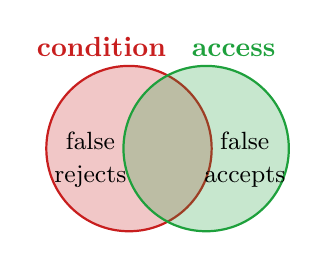
\begin{tikzpicture}[scale=0.7]
  \def\r{1.5}
  \coordinate (C1) at (-0.7,0);
  \coordinate (A1) at ( 0.7,0);
  \draw[fill=condred, fill opacity=0.25, draw=condred, thick] (C1) circle (\r);
  \draw[fill=accessgreen, fill opacity=0.25, draw=accessgreen, thick] (A1) circle (\r);
  \node[condred,above] at ($(C1)+(-0.5,1.5)$) {\textbf{condition}};
  \node[accessgreen,above] at ($(A1)+(0.5,1.5)$) {\textbf{access}};
  \node[align=center] at ($ (C1) + (-0.7,-0.2) $) {\small false\\ \small rejects};
  \node[align=center] at ($ (A1) + (0.7,-0.2) $) {\small false\\ \small accepts};
\end{tikzpicture}

\small\textbf{neither sound nor complete}
\end{minipage}
&
% 2: sound but not complete
\begin{minipage}{0.45\linewidth}\centering
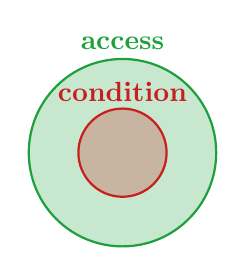
\begin{tikzpicture}[scale=0.7]
  \draw[fill=accessgreen, fill opacity=0.25, draw=accessgreen, thick] (0,0) circle (1.7);
  \draw[fill=condred, fill opacity=0.25, draw=condred, thick] (0,0) circle (0.8);
  \node[condred,above] at (0,0.75) {\textbf{condition}};
  \node[accessgreen,above] at (0,1.7) {\textbf{access}};
\end{tikzpicture}

\small\textbf{complete (no false rejects) but not sound}

\end{minipage}
\\[1em]

% 3: complete but not sound
\begin{minipage}{0.45\linewidth}\centering
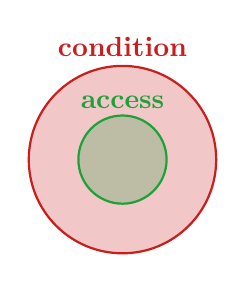
\begin{tikzpicture}[scale=0.7]
  \draw[fill=condred, fill opacity=0.25, draw=condred, thick] (0,0) circle (1.7);
  \draw[fill=accessgreen, fill opacity=0.25, draw=accessgreen, thick] (0,0) circle (0.8);
  \node[condred,above] at (0,1.7) {\textbf{condition}};
  \node[accessgreen,above] at (0,0.75) {\textbf{access}};
\end{tikzpicture}

\small\textbf{sound (no false accepts) but not complete}
\end{minipage}
&
% 4: sound and complete
\begin{minipage}{0.45\linewidth}\centering
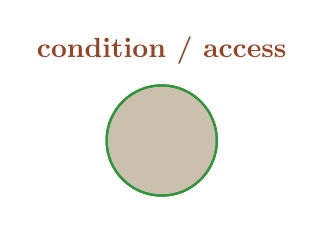
\begin{tikzpicture}[scale=0.7]
  \draw[fill=condred, fill opacity=0.25, draw=condred, thick] (0,0) circle (1.0);
  \draw[fill=accessgreen, fill opacity=0.18, draw=accessgreen, thick] (0,0) circle (1.0);
  \node[condred!70!accessgreen,above] at (0,1.2) {\textbf{condition / access}};
\end{tikzpicture}

\small\textbf{sound and complete}
\end{minipage}
\end{tabular}

\end{frame}


\begin{frame}[standout]
Group exercises
\end{frame}

%\agendaframe{group-exercises}


\begin{frame}{Random group assignments}
\begin{columns}
\begin{column}{0.33\textwidth}
Ashley, Isabelle: 5 \\ 
Bailey, Tanna: 12 \\ 
Blaisdell, Olyver: 2 \\ 
Brown, Ashton: 8 \\ 
Brown, Jonathan: 13 \\ 
Cardenas, Dominic: 6 \\ 
Cutler, George: 2 \\ 
Fabik, Roland: 10 \\ 
Fellows, Audrey: 7 \\ 
Fitzgerald, Ryan: 12 \\ 
Fuller, Ryan: 9 \\ 
Griffen, Clara: 4 \\ 
Grutsch, Tanner: 13 \\\end{column}
\begin{column}{0.33\textwidth}
Hager, Nathan: 9 \\ 
Horner, Jayden: 1 \\ 
Johnson, Jaret: 7 \\ 
Kintzel, Samantha: 1 \\ 
Lameres, Alexis: 6 \\ 
Lee, Holden: 6 \\ 
Mayala, Reece: 10 \\ 
McLean, Connor: 8 \\ 
Mcbride, Daniel: 9 \\ 
Miller, Maverick: 11 \\ 
Moss, Emily: 5 \\ 
Mousseau, Matthew: 11 \\ 
Neuman, Evan: 7 \\\end{column}
\begin{column}{0.33\textwidth}
Putnam, John: 3 \\ 
Ramos, Vydel: 13 \\ 
Rathbun, Jedidiah: 4 \\ 
Roberts, Matthew: 11 \\ 
Roller, Nathan: 10 \\ 
Ryan, Otis: 3 \\ 
Shevtsov, Timothy: 5 \\ 
Sinclair, Aidan: 3 \\ 
Smith, Charles: 4 \\ 
Stensland, Emma: 2 \\ 
Thiessen, Logan: 8 \\ 
Thompson, Jaiden: 12 \\ 
Vath, Ethan: 1 \\\end{column}
\end{columns}
\end{frame}



\begin{frame}{Group exercises}
\small 
\begin{enumerate}
 % Scheinerman
	\item It is a common mistake to confuse the following two statements (i) If A, then B and (ii) If B, then A. Find two conditions A and B such that statement (i) is true but statement (ii) is false. Then find two conditions A and B such that both statements are true. 
 % Scheinerman
	\item Consider these two statements: (i) If A, then B, (ii) If (not B), then (not A).  Under what circumstances are these statements true?  When are they false? Explain whether these statements are identical or not. \alert{[Note: (ii) is called the \textbf{contrapositive} of (i).]}
 % Norman Swartz
	\item (Challenge problem, from philosopher Norman Swartz.)  Is the following statement true or false, and why? \textit{A's-being-a-necessary-condition-for-B is both a necessary and sufficient condition for B's-being-a-sufficient-condition-for-A.}
\end{enumerate}
	
\end{frame}


\begin{frame}{Question 1: Solution}
$A \implies B$ but $B \centernot\implies A$: \\
A = I lived in Los Angeles \\
B = I lived in California. \\
\vfill 
$A \iff B$: \\
A = Valentine's Day is this month \\
B = This month is February. 
\end{frame}



\begin{frame}{Question 2: Solution}
\footnotesize
Recall from Slide \ref{slide:truth_table_for_if_A_then_B} that the truth table for the $\implies$ operator is given by  
\begin{center}
\begin{tabular}{cc|c}
X & Y & $\overbrace{X \implies Y}^{\text{If X, then Y}}$ \\
\hline 
T & T & T \\
T & F & F \\
F & T & T  \\
F & F & T  \\
\end{tabular}
\end{center}

Now we apply the $\implies$ operator to the results of the "\texttt{not}" operator (also written $\lnot$).
 
\begin{table}
\centering
\begin{tabular}{cc|ccc}
\multicolumn{2}{c}{\textbf{Orig. props.}} & \multicolumn{3}{c}{\textbf{New props.}} \\
A & B & $\overbrace{\lnot A}^{Y}$  & $\overbrace{\lnot B}^{X}$& $\overbrace{\lnot B \implies \lnot A}^{X \implies Y}$ \\
\hline 
T & T & \red{F}  & \red{F} & \green{T}\\
T & F & \red{F} & \green{T} &  \red{F}  \\
F & T & \green{T}  &  \red{F}  &  \green{T}  \\
F & F & \green{T} & \green{T} & \green{T}
\end{tabular}
\end{table}
%
Note that $\lnot B \implies \lnot A$ gives the same results as $A \implies B$ as on Slide \ref{slide:truth_table_for_if_A_then_B}.
\vfill 
\pause 
\bluetextbox{Remark: We've shown that a proposition is logically equivalent to its contrapositive.  So what?  Sometimes it's easier to verify the contrapositive version.} 
\end{frame}

\begin{frame}{Question 3: Solution}
The simplest way to see this is as follows:
\begin{itemize}
\item A's-being-a-necessary-condition-for-B can be expressed as $B \implies A$.
\item B's-being-a-sufficient-condition-for-A can be expressed as $B \implies A$. 
\item In other words, both propositions are the same: $B \implies A$. And a proposition is always necessary and sufficient for itself.  
\end{itemize}

\end{frame}

%\begin{frame}[standout]
%Appendix (feel free to skip)
%\end{frame}
%
%
%\begin{frame}{If and only if: How is it related to $==$?}
%\colorbox{red!30}{\textbf{Student question.}} How does iff relate to $==$ (the comparison operator in many programming languages)?
%
%\vfill \pause 
%
%\begin{myyellowbox}[title=Case Study]
%Consider propositions $A,B$ as binary-valued functions of $x$, which are elements of some set $\mathcal{X}$. For instance, perhaps 
%%
%\begin{align*}
%\mathcal{X} &= \set{\text{months since Labor Day was created (9/1882) until now}}  \\
%A(x) &= \text{month $x$ has Labor Day in it} \\
%B(x) &= \text{month $x$ is September} 
%\end{align*}
%%
%Then \texttt{A iff B} \alert{means}
%\[\text{for all} \; x \in \mathcal{X}, \qquad A(x) \explaintermbrace{written == in code}{=} B(x) \]
%\end{myyellowbox}
%
%\vfill \pause 
%
%\colorbox{green!30}{\textbf{Summary.}} iff means that $==$ returns True for \underline{all} cases of two propositions.
%%\begin{itemize}
%%	\item $==$ can be used to heck if two binary elements have the same truth value
%%	\item iff means that $==$ is true for \underline{all} cases of two propositions
%%\end{itemize}
%
%
%\end{frame}




\end{document}
